\chapter{Entwicklung}
\label{cha:Entwicklung}

Die im zweiten Kapitel beschriebenen theoretischen Grundlagen und auch praktischen Überlegungen zur Implementierung verteilter Systeme für Drohnenschwärme müssen jetzt in der Form eines Prototypen umgesetzt werden. Dies beginnt mit der Beschreibung der getroffenen Annahmen, da die Implementierung eines voll funktionsfähigen verteilten Systems in begrenzten Zeitrahmen mehr Zeitaufwand, Testing und Aufmerksamkeit für Details erfordert hätte. Dann folgt die Beschreibung des Gesamtsystems mit einer Gliederung der wichtigsten Komponenten. Anschließend wird die Implementierung des Raft-Algorithmus detailliert untersucht.

\section{Annahmen und Einschränkungen in der Entwicklung}

Die Implementierung jedes Systems erfordert Zeit, die auch exponentiell mit der Komplexität des Vorhabens steigt. Um einen realisierbaren Prototypen innerhalb einer überschaubaren Zeit zu implementieren, wurde eine Reihe von Annahmen getroffen.

\subsection{Scala als Programmiersprache}

Als Programmiersprache für die Implementierung des Prototypen wurde Scala verwendet. Scala ist eine \textit{Universalsprache}, die sowohl objektorientierte Programmierung als auch funktionale Programmierung unterstützt. Die Sprache ist statisch typisiert. Der Scala-Quellcode wird in Java Bytecode kompiliert, sodass der resultierende ausführbare Code auf der Java Virtual Machine (JVM) ausgeführt werden kann. Scala bietet Interoperabilität mit Java. Im Gegensatz zu Java verfügt Scala über viele Eigenschaften funktionaler Programmiersprachen, wie beispielsweise Scheme, Standard ML und Haskell, einschließlich Currying, Immutability (Unveränderlichkeit), die Lazy Evaluation (bequeme oder auch faule Auswertung) und Pattern Matching. Es verfügt ebenfalls über ein fortschrittliches Typsystem, das algebraische Datentypen, Kovarianz und Kontravarianz sowie anonyme Typen unterstützt. Andere Funktionen von Scala, die in Java nicht vorhanden sind, sind das Überladen von Operatoren, optionale Parameter und benannte Parameter.

Laut \textit{"Github Language Stats"} (Stand 23.12.2020) erreichte Scala bei der Anzahl an Pull-Requests den elften Platz und überholte somit Programmiersprachen wie Rust, Kotlin, Swift und Haskell.

Für die Implementierung eines Produktivsystems, welches auf einer Drohne läuft und auch Leistungsanforderungen des Betriebssystems einer Drohne erfüllt, wären solche Systemprogrammiersprachen wie C++ oder Rust geeignet. Scala ermöglicht aufgrund seiner Simplizität ein schnelles Prototyping, das Aktorsystem (actors system) dieser Programmierungssprache mit zahlreichen Eigenschaften hat einen guten Ruf bekommen und die Integration des Aktorsystems mit dem Play-Web-Frameworks machen Scala zu einer guten Option für die Implementierung eines Prototypen.

\subsection{Akka für das Implementieren verteilter Systeme}

Den größten Vorteil von Scala bietet das Aktorsystem, genauer gesagt das Aktorsystem der Akka-Bibliothek. Die Verwendung von Akka macht die Erstellung der Infrastruktur für ein Aktorsystem und das Schreiben des Low-Level-Codes, der zur Steuerung des grundlegenden Verhaltens erforderlich ist, überflüssig.

Ein Aktor in Akka hat immer einen Elternknoten und alle Knoten sind Kinder des Guardian-Knotens, der beim Start eines Aktorsystems erstellt wird. Eine Instanz des ActorSystems dient zur Kommunikation mit dem Aktorsystem, zur Erstellung neuer Aktoren, zur Adressierung und zur Verwaltung des Kontexts. Eine reibungslose Kommunikation zwischen den Aktoren ist nur innerhalb des Systems möglich. Wenn eine andere Softwarekomponente einen Aktor innerhalb des Aktorsystems aufrufen möchte, muss diese Anfrage mittels Adapter übersetzt werden. Dasselbe gilt für Antworten des Aktorsystems. Die Kommunikation im Aktorsystem ist immer asynchron.

Bevor der erste Aktor gestartet wird, hat Akka bereits 2 Aktoren erstellt. Die Namen dieser eingebauten Aktoren enthalten \textit{"guardian"} (Wächter). Die Guardian-Aktoren umfassen:

\begin{enumerate}
	\item "/" - der sogenannte Root-Guardian. Das ist das übergeordnete Element aller Aktoren im System und das letzte, das angehalten wird, wenn das System stoppt.
	
	\item "/system" - der System-Guardian. Das ist ein Aktor, der das System aufrechterhält. Akka oder andere Bibliotheken, die auf Akka basieren, können Aktoren im Systemnamespace erstellen.
	
	\item "/user " - der Benutzer-Guardian. Das ist der Aktor, der alle anderen Aktoren einer Anwendung startet.
\end{enumerate}

Struktur der Guardian Aktoren wird in der Abbildung \ref{fig:akkaActors} dargestellt.

\begin{figure}
	\centering
	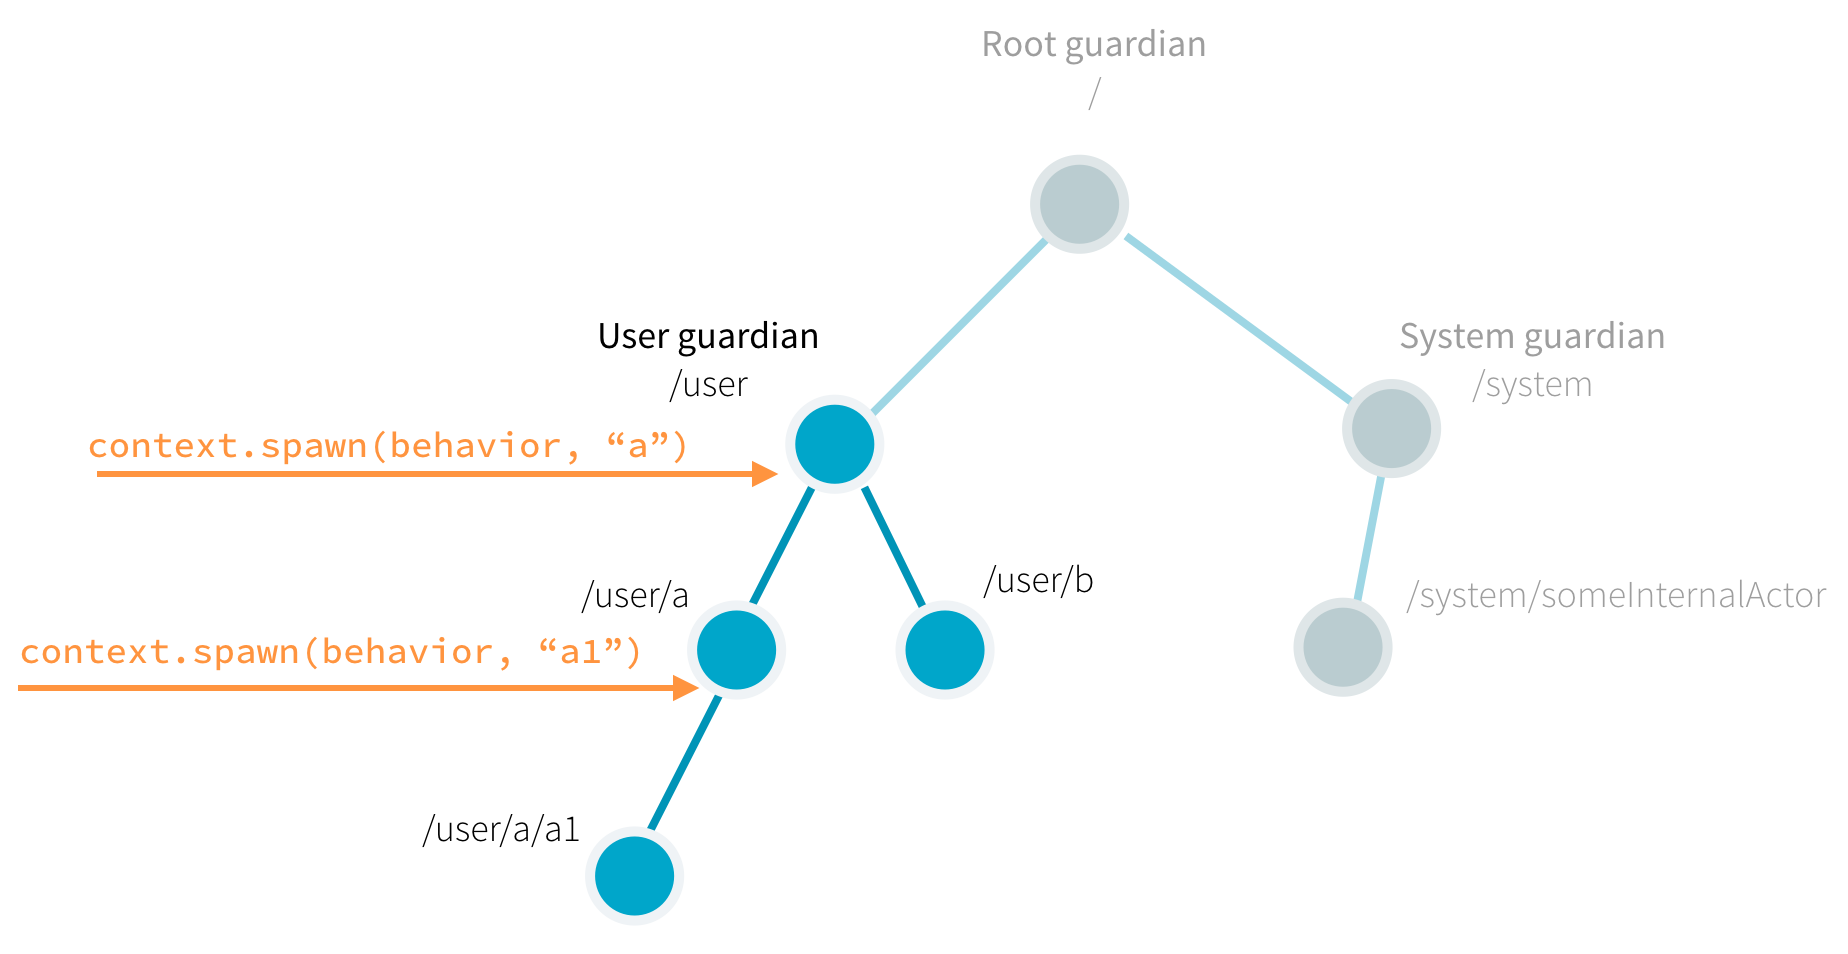
\includegraphics[width=0.7\linewidth]{images/3_akka_actors}
	\caption{Beispiel eines Aktorsystems zusammen mit den Aktoren, die von Akka standardmäßig erstellt werden.}
	\label{fig:akkaActors}
\end{figure}

Anwendung des Akka Aktorsystems und seiner Module bringt folgende Vorteile für verteilte Systeme:

\begin{description} 
	\item[Protokollunabhängigkeit.] Standardmäßig bietet Akka eine Integration mit HTTP, aber mittels Konnektoren (Adapters anders gesagt) kann man auch problemlos über MQTT, AMQP, JMS (Java Message Service) und gRPC kommunizieren.
	
	\item[Verteilte Aktoren.] Akka Remoting ermöglicht Aktoren, die auf verschiedenen Rechnern laufen, Nachrichten nahtlos auszutauschen. Dank des Aktormodells sieht ein ferner und lokaler Nachrichtenversand gleich aus. Es bietet die Basis, auf der das Cluster-Subsystem aufgebaut ist.
	
	\item[Unterstützung von Clusters.] Wenn es in einem verteilten System eine Reihe von Aktoren gibt, die zusammenarbeiten, um eine Aufgabe zu lösen, muss das System auf eine bestimmte Weise aufgebaut und gesteuert werden. Während Akka-Remoting das Problem der Adressierung und Kommunikation zwischen Komponenten eines verteilten Systems löst, bietet Clustering die Möglichkeit, diese Knoten in der Form eines Metasystems mit einem Mitgliedschaftsprotokoll zu organisieren. Das ist ein Teil der Kontrollebene eines Clusters.
	
	\item[Sharding (horizontale Fragmentierung).] Sharding ist ein Vorgehen, das verwendet wird, um eine große Anzahl von Aktoren auf Knoten eines Clusters aufzuteilen und sie auch auf andere Knoten zu verschieben, wenn andere Knoten abstürzen oder unerreichbar werden.
\end{description}

Akka verfügt über mehrere Kommunikationspatterns. Einige von ihnen sind für Aktorsysteme spezifisch und dienen dazu, ein erklärbares und skalierbares System zu entwickeln. Diese spezifische Patterns sind z.B:

\begin{enumerate}
	\item Zusendung des Ergebnisses eines Futures (in der Fußnote erklären, was ein Future ist) an sich selbst
	
	\item Per-Session-Child-Actor (Erstellung eines Aktors je Sitzung) in dem ein Elternknoten einen Kindknoten erstellt. Der Kindknoten stellt eine asynchrone Operation dar, die allen anderen Aktoren abfragen muss, das Ergebnis dem Elternknoten zur Verfügung stellt und sich anschließen stoppt. Die Erstellung eines neuen Aktors für jede Anfrage kann verschwenderisch klingen (vor allem in einem eingebetteten System), die Erstellung eines neuen Aktors erfordert allerdings keine Ressourcen des Betriebssystems und ist deswegen sehr billig.
\end{enumerate}

Patterns, die bei der Implementierung des Raft-Algorithmus eingesetzt wurden, sind:

\begin{description} 
	\item[Fire and Forget (Tell-Ansatz).] Fire-And-Forget ist der fundamentale Weg für die Kommunikation zwischen Aktoren. "Tell" ist asynchron, was bedeutet, dass die Methode in einem anderen Thread gestartet wird. Nachdem der Befehl ausgeführt wurde, gibt es keine Garantie, dass die Nachricht noch vom Empfänger verarbeitet wurde. Das bedeutet auch, dass es keine Möglichkeit gibt herauszufinden, ob die Nachricht empfangen wurde, die Verarbeitung erfolgreich war oder fehlgeschlagen ist. Fire-And-Forget ist so üblich bei Akka, dass es einen speziellen symbolischen Namen hat: “!” (Ausrufezeichen). Der Versand einer Nachricht hätte dann so ausgesehen “actor ! message”.
	
	\item[Request-Response mit einer oder mehreren Antworten.] Mehrere Interaktionen erfordern eine oder mehrere Antworten. Um die Antwort zu erhalten muss der Absender seine Adresse in der Nachricht mitschicken.
	
	\item[Request-Response mit einer einzelnen Antwort (Ask-Ansatz).] Wenn für eine Anfrage genau eine Antwort erwartet wird, verwendet man Ask-Anfragen. Eine Ask-Anfrage hat ebenfalls eine spezielle Bezeichnung: “?”. Da alle Kommunikationen im Aktorsystem asynchron sind, darf man einen Aktor mit der Ask-Anfrage nicht blockieren. Die Antwort wird asynchron empfangen und in einen Callback übergeben, der bei der Absendung der Ask-Anfrage erstellt sein soll.
	
	\item[Interaktion mit externen Komponenten.] Da Aktoren standardmäßig nur mit anderen Aktoren innerhalb eines Aktorsystems kommunizieren können, braucht man eine Brücke für die Außenwelt. Eine der möglichen Lösungen ist Future. Dies ist eine Abstraktionsschicht über übliche Callbacks und stellt Ergebnis einer asynchronen Operation dar. Ein Future wird normalerweise von einem Promise erstellt, der ein Proxy zwischen einer Rechenoperation und dem Future (dem asynchronen Ergebnis) darstellt.
	
	\item[Scheduling messages to self (Zusendung an sich selbst zu planen).] Standardmäßig erlaubt Akka einem Aktor Nachrichten an sich selbst zu schicken. Dadurch kann man Timeouts implementieren, auf denen Paxos und andere Algorithmen für verteilte Systeme beruhen.
\end{description}

Das Kommunikationsmuster eines Knotens mit anderen Knoten und dessen Verhalten kann sich mit der Zeit ändern. Das passiert, wenn ein Knoten mehr Funktionen bzw. andere Funktionen in der Hierarchie übernimmt, beispielsweise die Funktion eines Beobachters und Workers gleichzeitig, oder die Funktion eines Beobachters und eines Response Aggregators. Da ein Aktor als solcher einen Zustandsautomaten darstellt, der beliebig kompliziert sein kann, führt es zu einem Zustandsautomaten mit verschachtelten Zuständen. Um diese Überlappung von Funktionen und Komplexitäten aufzulösen, gibt es bei Akka zwei Herangehensweisen: die erste klassische Methode, die sich vorzüglich bewährt hat, ist die Zersetzung eines Aktors in mehrere Aktoren. Die zweite Methode ist die Auswechslung von \textit{Behaviors} (Verhalen). Ein Behavior repräsentiert einen Übergang in einen neuen globalen Zustand. Ein solcher globaler Übergang wäre in Raft der Übergang vom Follower-Zustand zum Leader-Zustand. Ein Aktor dient in diesem Fall als Container (Behälter) für Behaviors mit einem anfänglichem Verhalten. Behaviors entscheiden selbstständig, was das nächste Behavior ist und ob ein Behavior zu einem bestimmten Zeitpunkt überhaupt ausgetauscht werden soll. Wenn ein Behavior ausgewechselt wird, bleibt der Container (also Aktor) intakt. Einen Übergang von Zuständen innerhalb eines Aktors könnte man beim Raft-Algorithmus wie in der Abbildung \ref{fig:stateTransition} darstellen.

\begin{figure}
	\centering
	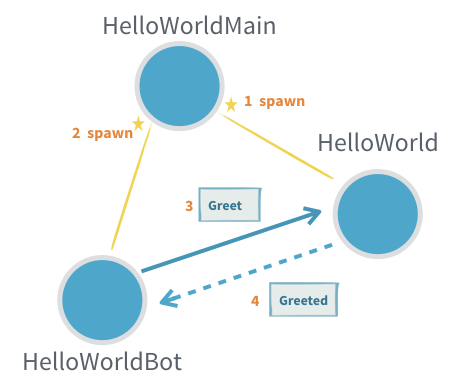
\includegraphics[width=0.7\linewidth]{images/4_state_transition}
	\caption{Übergang von Zuständen im Raft-Algorithmus}
	\label{fig:stateTransition}
\end{figure}

Dadurch, dass Akka viele wichtige Bausteine für den Aufbau verteilter Systeme auf Mikroebene (automatische Serialisierung und Deserialisierung von Nachrichten, Timers, Austausch von Behaviors) und Makroebene (Protokollunabhängigkeit, Unterstützung verteilter Aktoren und Clusters von Aktoren) bietet, ist es für die Implementierung eines verteilten Systems besonders gut geeignet.

\subsection{Einschränkungen bei der Implementierung eines verteilten Systems mit Akka}

Wie es schon im zweiten Kapitel festgestellt wurde, folgt das Aktorsystem dem Prinzip \textit{"let it crash"}, bei dem ein Kindknoten seinem Elternknoten über Ausnahmesituationen Bescheid gibt, sodass der letzte Knoten alle dieser Situationen auflöst. Wenn ein Elternknoten eine Ausnahmesituation nicht auflösen kann, delegiert er seinem Elternknoten die Verantwortung für die Situation. Dadurch entsteht ein Baum von Aktoren, in dem ein übergeordneter Knoten einen untergeordnete Knoten beobachtet und verwaltet. Das bedeutet, dass alle fehlerhaften Operationen in Blättern des \textit{Observation-Tree} (Beobachtungsbaum) konzentriert werden. Je näher ein Aktor der Wurzel des Baumes ist, desto weniger Ausnahmesituationen werden für ihn möglich sein. Die Robustheit der Hierarchie wird durch die Abgrenzung von fehlerhaften Operationen in mehreren kleinen Blattaktoren erreicht. Das stimmt mit dem bekannten Zitat des Erfinders des Aktorsystems Tony Hoare überein:

"There are two ways of constructing a software design: One way is to make it so simple that there are obviously no deficiencies and the other way is to make it so complicated that there are no obvious deficiencies."

Das Konzept der Verschiebung des kritischen Codes in äußere Knoten des Baumes nennt man \textit{Error-Kernel} (der Kernel der Fehler).

Bei Aktorsystemen ist es untypisch, wenn eine Hierarchie weniger als zwei oder drei Schichten enthält. Für eine Drohne könnte eine Hierarchie so ausschauen, wie es in der Abbildung \ref{fig:hierarchy1} dargestellt wird.

\begin{figure}
	\centering
	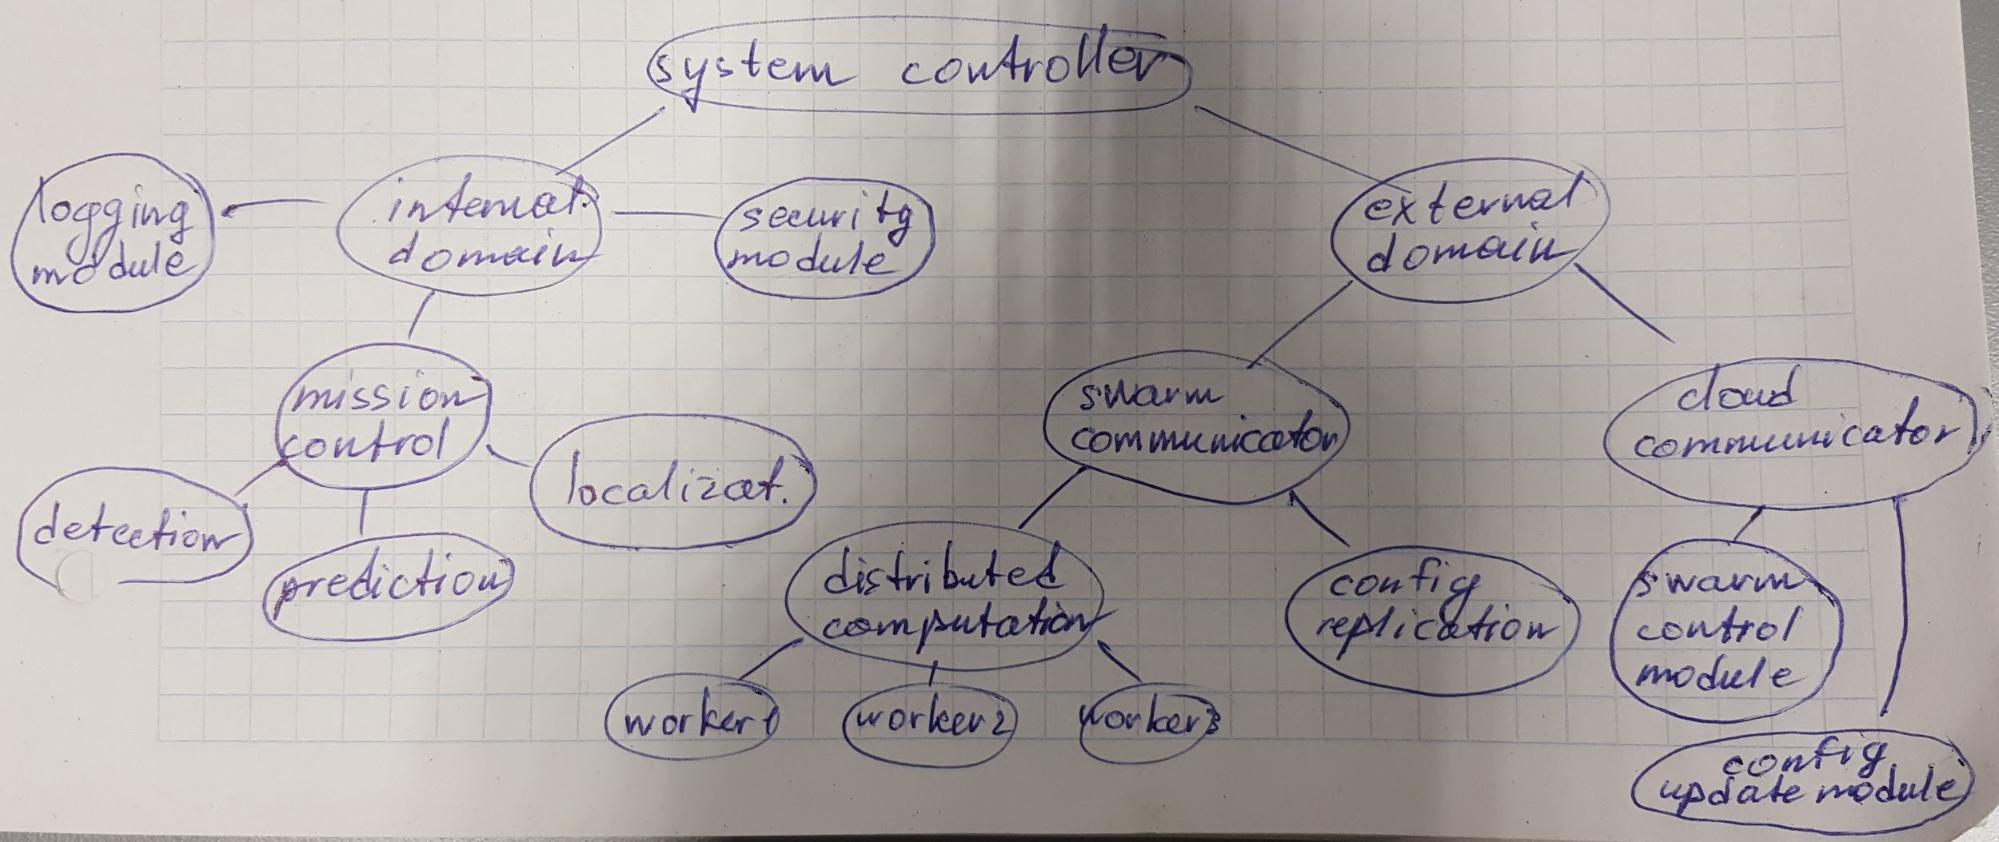
\includegraphics[width=0.7\linewidth]{images/5_hierarchy_1}
	\caption{Möglicher Aufbau eines Systems für Drohnensteuerung mithilfe Aktorsystems.}
	\label{fig:hierarchy1}
\end{figure}

Der Knoten, der für die Replikation des Zustandes zwischen den Drohnen verantwortlich ist und den Raft-Algorithmus implementiert würde, wäre \textit{Configuration-Replication} (die Replikation der Konfiguration, abgbildet rechts unten). Aufgrund des Aufbaus eines Prototypen war die Hierarchie des Raft-Algorithmus flach gehalten und nur mit zwei Schichten implementiert: eine Schicht des Clients, der Anfragen an das System entgegennimmt, und die andere Schicht der Raft Knoten. Die Hierarchie entspricht der Abbildung \ref{fig:hierarchy2}.

\begin{figure}
	\centering
	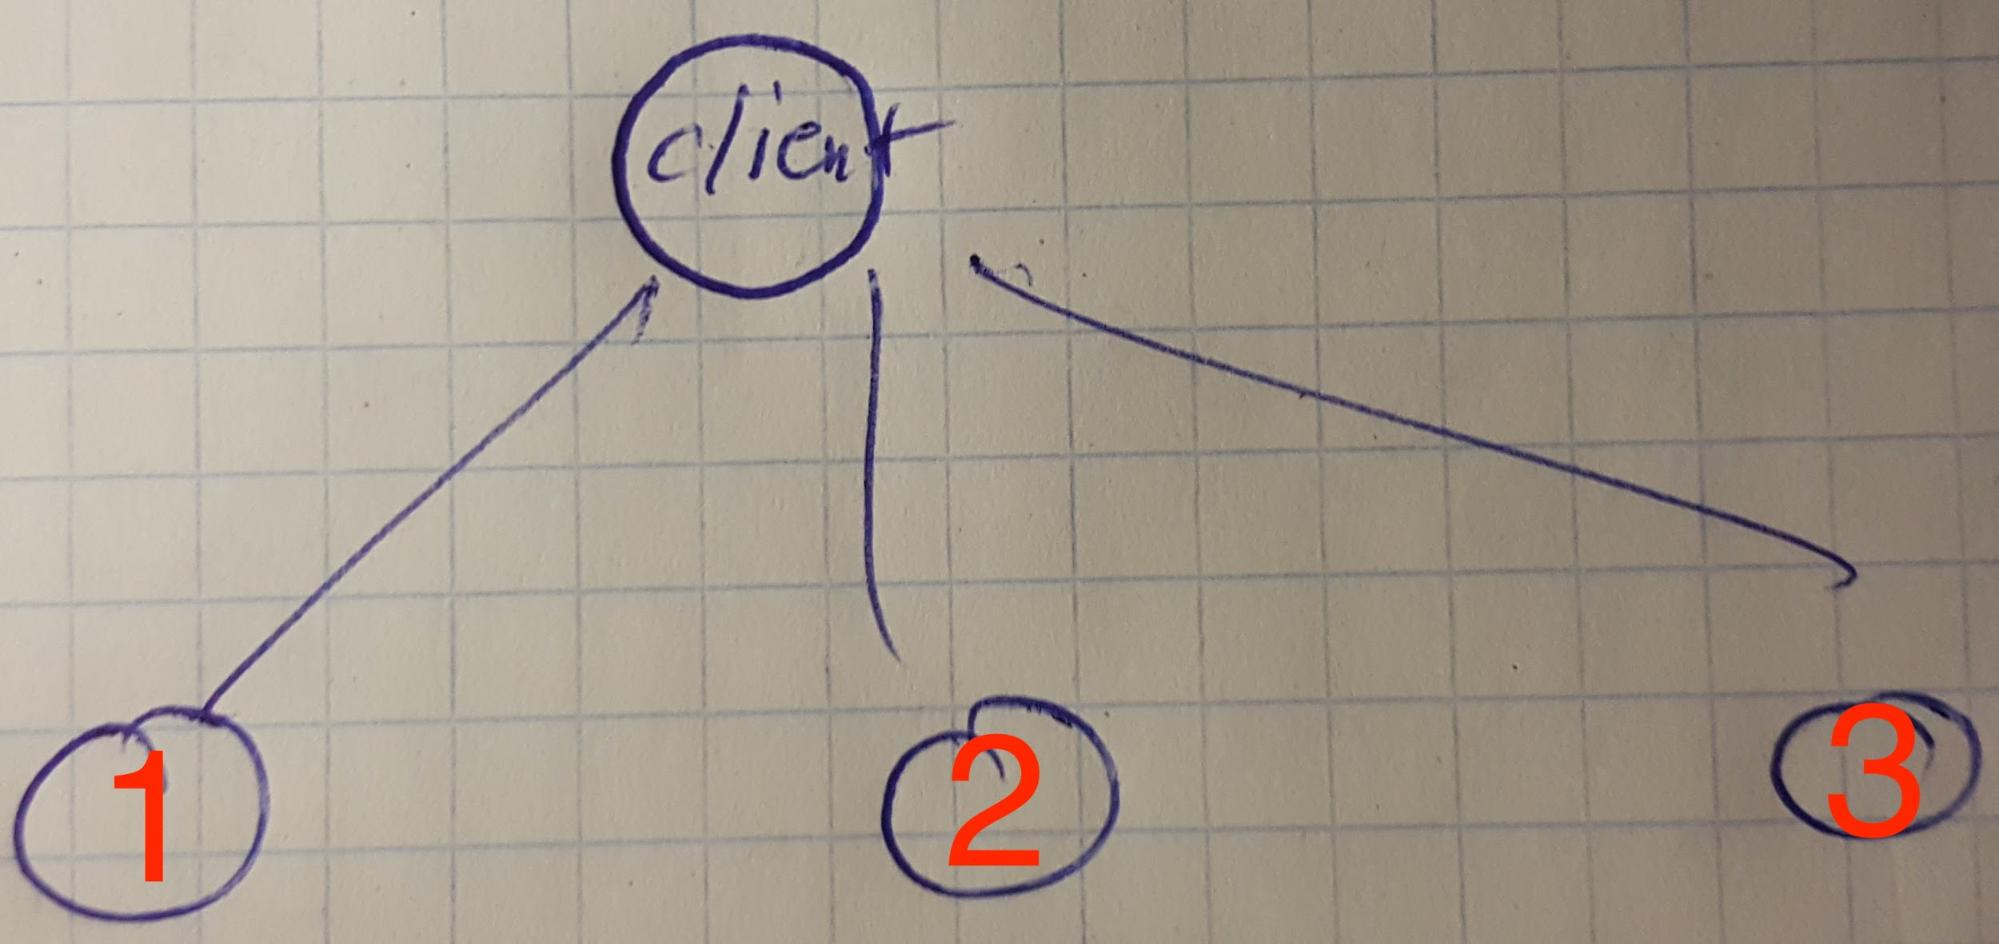
\includegraphics[width=0.7\linewidth]{images/6_hierarchy_2}
	\caption{Möglicher Aufbau eines Systems für Drohnensteuerung mithilfe Aktorsystems.}
	\label{fig:hierarchy2}
\end{figure}

Die Knoten 1, 2 und 3 entsprechen den Configuration-Replication-Knoten der ersten drei Drohnen. Der Client ist der Knoten, der sich in der Cloud befindet und als Proxy für den Drohnenschwarm dient. Der zu replizierende Wert wird vom Client an einen Knoten geschickt, der die Leader-Rolle im Cluster erfüllt und dann anschließend ohne Beteiligung des Clients laut Raft-Algorithmus zwischen Knoten repliziert.

\subsection{Annahmen für Server und Frontend des Prototypen}

Heutzutage werden vor allem zwei Frameworks für die Entwicklung von Webdiensten auf der JVM verwendet: Jakarta EE und Spring. Scala bietet ein eigenes Framework namens Play. Dies ist für die Entwicklung von  MVC- (Model View Controller) und REST-Diensten (Representational State Transfer) geeignet. Play beruht auf Akka-HTTP. Akka-HTTP ist kein Webframework, sondern ein allgemeines Werkzeug in der Akka Werkzeugpalette, um HTTP basierte Dienste aufrufen und HTTP-Anfragen beantworten zu können.

Play bietet folgende Vorteile:

\begin{enumerate}
	\item standardmäßige Unterstützung von Scala
	
	\item einfache integration mit Akka Aktorsystem
\end{enumerate}

Für die Entwicklung des Frontends wurde React verwendet. React ist ein Framework von Facebook, das eine schnelle (im Vergleich mit reinen JavaScript und HTML) Entwicklung von Webanwendungen ermöglicht.

\section{Beschreibung der Teilkomponenten und Schnittstellen des Systems}











\textit{}

\begin{table} \centering
	\begin{tabular}{|P{3cm}|P{3cm}|P{3cm}|P{3cm}|P{3cm}|} 
		\hline
		&  \textbf{Aktormodell} & \textbf{CSP} & \textbf{Funktionale Programmierung} & \textbf{Threads und Mutex}\\
		
		\hline
		Primär Fokus & Fehlertoleranz und verteiltes Rechnen & Flexibilität und Ausdruckskraft & Nebeneffektefreiheit durch Immutability & Effizienz und breite Anwendbarkeit\\
		
		\hline
	\end{tabular}
	\caption{Vergleich von Concurrency Modellen.}
	\label{tab:123}
\end{table}

\begin{description} 
	\item[.] 
	
	\item[.] 
	
	\item[.] 
\end{description}

\begin{enumerate}
	\item 
	
	\item 
	
	\item 
	
	\item 
\end{enumerate}